

We presents a new automated method for relative termination of double-pushout (DPO) graph rewriting systems with injective rules~\cite{corradini1997algebraic,habel2001double,konig2018atutorial}~\footnote{This work resulted in a publication at the 18th International Conference on Graph Transformation (ICGT 2025)~\cite{qiu2025termination_icgt}.}. 

The method, based on the interpretation method framework~\cite{nipkow1998term,contejean2005mechanically}, works as follows. Let \( \mathbb{X} \) denote a fixed set of graphs. We assign weights (natural numbers) to monomorphisms from graphs in \( \mathbb{X} \), and define the weight of a graph $G$ as the sum of the weights of all monomorphisms from graphs in \( \mathbb{X} \) to $G$. 

Let $\mathcal{A}$ and $\mathcal{B}$ be sets of DPO rewriting rules. Let $X \in \mathbb{X}$ and $G \Rightarrow H$ be a rewriting step defined by the double-pushouts diagram shown below. 
% in Figure~\ref{fig:subgraph_counting:general_rewriting_step_sdfsl}.
% \begin{figure}[H]
%     \centering
\begin{center}
 \resizebox{0.4\textwidth}{!}{
     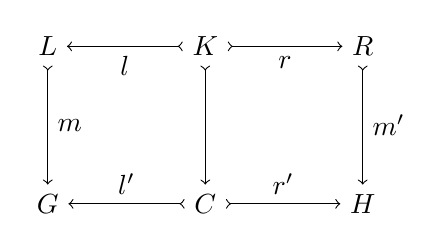
\begin{tikzpicture}
            % [node distance=15mm]
            \node (I) at (0,0) {$K$};
            \node (L)  at (-2,0) {$L$};
            \node (R)  at (2,0) {$R$};
            \node (G)  at (-2,-2) {$G$};
            \node (C)  at (0,-2) {$C$};
            \node (H)  at (2,-2) {$H$};
            \draw [>->] (I) to  node [midway,below] {$l$} (L);
            \draw [>->] (I) to  node [midway,below] {$r$} (R);
            \draw [>->] (L) to node [midway,right] {$m$} (G);
            \draw [>->] (I) to  node [midway,right] 
            % {$u$}
            {} (C);
            \draw [>->] (R) to  node [midway,right] 
            {$m'$}
            (H);
            \draw [>->] (C) to node [midway,above] {$l'$} (G);
            \draw [>->] (C) to node [midway,above] 
            {$r'$} 
            (H);
            % \node [at=($(I)!.5!(G)$)] {\normalfont PO};
            % \node [at=($(I)!.5!(H)$)] {\normalfont PO};
        \end{tikzpicture}
    }
%     \caption{}
%     \label{fig:subgraph_counting:general_rewriting_step_sdfsl}
% \end{figure}
    \end{center}

For a monomorphism from $X$ to $G$, its image falls into exactly one of the following three mutually exclusive cases:
\begin{enumerate}
    \item the image may be fully included in $m(L)$;
    \item the image may be fully included in $l'(C)$; 
    \item the image may be neither fully included in $m(L)$ nor fully included in $l'(C)$.
\end{enumerate} 
 Similary, for a monomorphism from $X$ to $H$, its image falls into exactly one of the following three mutually exclusive cases:
 \begin{itemize}
    \item the image may be fully included in $m'(R)$;
    \item the image may be fully included in $r'(C)$;
    \item the image may be neither fully included in $m'(R)$ nor fully included in $r'(C)$.
 \end{itemize}
  The number of monomorphisms from $X$ to $G$ whose image is fully included in $m(L)$ can be precisely calculated, as can the number of monomorphisms from $X$ to $H$ whose image is fully included in $m'(R)$. Moreover, the number of monomorphisms from $X$ to $G$ equals to the that of monomorphisms to $H$. 

To estimate the change in weight when applying a rewriting rule, we focus on 
the monomorphisms in the third case. Specifically, our technique requires that, for every graph $X$ in $\mathbb{X}$ and every rewriting step $G \Rightarrow H$ using a rule from $\mathcal{A}$ or $\mathcal{B}$, there is an injective mapping from the set of monomorphisms $x : X \to H$ (where $\opn{Im}(x)$ is neither fully included in the right-hand side graph nor fully included in the context) to the set of monomorphisms from $y : X \to G$ (where $\opn{Im}(y)$ is neither fully included in the left-hand side graph nor fully included in the context). 

Suppose, additionally, that the following conditions hold: 
\begin{itemize}
    \item For every rule in \( \mathcal{A} \), the left-hand side graph's weight is strictly greater than the right-hand side graph's weight; 
    \item For every rule in \( \mathcal{B} \), the left-hand side graph's weight is greater than or equal to the right-hand side graph's weight.
\end{itemize}

Under these conditions, rewriting steps using rules in \( \mathcal{A} \) strictly decrease the weights of the host graphs, while rewriting steps using rules in \( \mathcal{B} \) do not increase them.
Consequently, the rewriting rules in \( \mathcal{A} \) can only be applied finitely many times, since the weight of a finite graph is a natural number and strictly decreases with each rewriting step using a rule in \( \mathcal{A} \), the process must terminate after a finite number of iterations.  
% Chapter~\ref{chap:subgraph_counting} presents an new automated method for relative termination~\cite{geser1990relative} of double-pushout (DPO) graph rewriting systems with injective rules~\cite{corradini1997algebraic,habel2001double,konig2018atutorial}.
%  The method, based on the interpretation method framework~\cite{nipkow1998term}, works as follows. Let \( \mathbb{X} \) denote a fixed set of graphs. We assign weights (natural numbers) to monomorphisms from graphs in \( \mathbb{X} \), and define the weight of a graph $G$ as the sum of the weights of all monomorphisms from graphs in \( \mathbb{X} \) to $G$. 

% Let $\mathcal{A}$ and $\mathcal{B}$ be sets of DPO rewriting rules. Let $X \in \mathbb{X}$ and $G \Rightarrow H$ be a rewriting step defined by the double-pushouts diagram in Figure~\ref{fig:subgraph_counting:general_rewriting_step_sdfsl}.
% \begin{figure}[H]
%     \centering
%  \resizebox{0.4\textwidth}{!}{
%      \begin{tikzpicture}
%             % [node distance=15mm]
%             \node (I) at (0,0) {$K$};
%             \node (L)  at (-2,0) {$L$};
%             \node (R)  at (2,0) {$R$};
%             \node (G)  at (-2,-2) {$G$};
%             \node (C)  at (0,-2) {$C$};
%             \node (H)  at (2,-2) {$H$};
%             \draw [>->] (I) to  node [midway,below] {$l$} (L);
%             \draw [>->] (I) to  node [midway,below] {$r$} (R);
%             \draw [>->] (L) to node [midway,right] {$m$} (G);
%             \draw [>->] (I) to  node [midway,right] 
%             % {$u$}
%             {} (C);
%             \draw [>->] (R) to  node [midway,right] 
%             {$m'$}
%             (H);
%             \draw [>->] (C) to node [midway,above] {$l'$} (G);
%             \draw [>->] (C) to node [midway,above] 
%             {$r'$} 
%             (H);
%             % \node [at=($(I)!.5!(G)$)] {\normalfont PO};
%             % \node [at=($(I)!.5!(H)$)] {\normalfont PO};
%         \end{tikzpicture}
%     }
%     \caption{}
%     \label{fig:subgraph_counting:general_rewriting_step_sdfsl}
% \end{figure}

% For a monomorphism from $X$ to $G$, its image falls into exactly one of the following three mutually exclusive cases. First, the image may be fully included in $m(L)$. Second, the image may be fully included in $l'(C)$; Third, the image may be neither fully included in $m(L)$ nor fully included in $l'(C)$. Similary, for a monomorphism from $X$ to $H$, its image falls into exactly one of the following three mutually exclusive cases. First, the image may be fully included in $m'(R)$. Second, the image may be fully included in $r'(C)$; Third, the image may be neither fully included in $m'(R)$ nor fully included in $r'(C)$. The number of monomorphisms from $X$ to $G$ whose image is fully included in $m(L)$ can be precisely calculated, as can the number of monomorphisms from $X$ to $H$ whose image is fully included in $m'(R)$. Moreover, the number of monomorphisms from $X$ to $G$ equals to the that of monomorphisms to $H$. 

% To estimate the change in weight when applying a rewriting rule, we focus on 
% the monomorphisms in the third case. Specifically, our technique requires that, for every graph $X$ in $\mathbb{X}$ and every rewriting step $G \Rightarrow H$ using a rule from $\mathcal{A}$ or $\mathcal{B}$, there exists an injective mapping from the set of monomorphisms $x : X \to H$ (where $\opn{Im}(x)$ is neither fully included in the right-hand side graph nor fully included in the context) to the set of monomorphisms from $y : X \to G$ (where $\opn{Im}(y)$ is neither fully included in the left-hand side graph nor fully included in the context). 

% Suppose, additionally, that the following conditions hold: (i) For every rule in \( \mathcal{A} \), the left-hand side graph's weight is strictly greater than the right-hand side graph's weight; (ii) For every rule in \( \mathcal{B} \), the left-hand side graph's weight is greater than or equal to the right-hand side graph's weight. 

% Under these conditions, rewriting steps using rules in \( \mathcal{A} \) strictly decrease the weights of the host graphs, while rewriting steps using rules in \( \mathcal{B} \) do not increase them.
% Consequently, the rewriting rules in \( \mathcal{A} \) can only be applied finitely many times, since the weight of a finite graph is a natural number and strictly decreases with each rewriting step using a rule in \( \mathcal{A} \), the process must terminate after finitely many iterations.  
 
% Our method proves termination for systems such as the one inExample~\ref{subgraph_counting:ex_contrib_variant}, which prior interpretation-based approaches~\cite{zantema2014termination,bruggink2014termination,bruggink2015proving,
% endrullis2024generalized_arxiv_v2,
% overbeek2024termination_lmcs} cannot handle. 
% We also provide an implementation of our technique.  
   
This chapter is organized as follows.
We first define the weight of a graph in~\textsection~\ref{subgraph_counting:sec:interpretation}. 
Using this definition, we outline the general approach and identify the key challenge in~\textsection~\ref{subgraph_counting:sec:general_idea} and introduce the concept of non-increasing rules in \textsection~\ref{subgraph_counting:sec:non-increasing}. 
A solution to the challenge is then proposed in~\textsection~\ref{subgraph_counting:sec:solution_to_the_key_challenge}, culminating in our termination criterion in~\textsection~\ref{subgraph_counting:sec:termination}.
\textsection~\ref{subgraph_counting:sec:examples} illustrates the method with some examples.
\textsection~\ref{subgraph_counting:sec:related_work} compares our approach with some existing methods.
Finally,~\textsection~\ref{subgraph_counting:sec:conclusion} concludes with remarks and future research directions. Proofs of some propositions, lemmas, and theorems of this chapter
 have been moved to Appendix~\ref{subgraph_counting:sec:appendix} to improve readability.